\hypertarget{guns-bombs-and-buses-going-really-fast}{%
\section{Guns, bombs and buses going really
fast}\label{guns-bombs-and-buses-going-really-fast}}

\begin{figure}[!ht]
  \begin{adjustwidth}{-\oddsidemargin-1in}{-\rightmargin}
    \centering
    
\includegraphics[trim={0 7cm 0 1cm,}, clip, width=\paperwidth]{./S01/img/19/guns-bombs-and-buses-going-really-fast.png}
    % \caption{Guns, bombs and buses going really fast\label{fig:guns-bombs-and-buses-going-really-fast}}
  \end{adjustwidth}
\end{figure}

\begin{tcolorbox}[enhanced,center upper,
    drop fuzzy shadow southeast, boxrule=0.3pt,
    lower separated=false, breakable,
    colframe=black!30!dialogoBorder,colback=white]
\begin{minipage}[c]{0.16\linewidth}
  \raisebox{\dimexpr-\height+\ht\strutbox\relax}{
    \centering 
\includegraphics[width=1.4cm]{./assets/img/phoebe.png}
  }
   & \centering \scriptsize{Phoebe}
\end{minipage}
\hfill
\begin{minipage}[c]{0.8\linewidth}
  \textbf{- I'm sorry it wasn't one of those movies with guns and bombs and buses going really fast.}\\
  - Desculpe se não foi um daqueles filmes com armas e bombas e ônibus em alta velocidade.
\end{minipage}
\end{tcolorbox}

Na volta do cinema os rapazes estão insatisfeitos e Phoebe descreve o
filme \emph{Speed} (1994), em que a premissa do filme é que uma bomba
foi plantada num ônibus e ela irá explodir caso o veículo ande abaixo de
um limite de velocidade. No decorrer do filme o motorista é baleado e
uma passageira assume o volante. No Brasil o filme ficou conhecido como
\emph{Velocidade Máxima}.\footnote{\sloppy Speed - IMDB. \url{https://www.imdb.com/title/tt0111257/?ref_=nv_sr_srsg_0}}

\begin{figure}
  \centering
  \begin{tikzpicture}
    \node [inner sep=0pt] at (0,0) {
      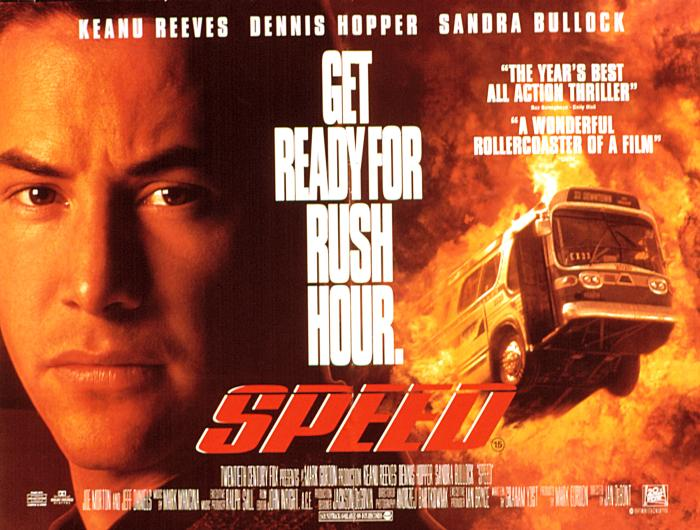
\includegraphics[width=0.6\textwidth,keepaspectratio]{./S01/img/19/speed-poster.jpg}
    };
    \draw [white, rounded corners=\ClipSep, line width=\ClipSep]
    (current bounding box.north west) --
    (current bounding box.north east) --
    (current bounding box.south east) --
    (current bounding box.south west) -- cycle
    ;
    \end{tikzpicture}
    \caption{Speed - Poster\label{fig:speed-poster}}
\end{figure}

\hypertarget{lou-grant-or-hugh-grant}{%
\section{Lou Grant or Hugh Grant}\label{lou-grant-or-hugh-grant}}

\begin{figure}[!ht]
  \begin{adjustwidth}{-\oddsidemargin-1in}{-\rightmargin}
    \centering
    
\includegraphics[trim={0 6cm 0 2cm,}, clip, width=\paperwidth]{./S01/img/19/lou-grant-or-hugh-grant.png}
    % \caption{Lou Grant or Hugh Grant\label{fig:lou-grant-or-hugh-grant}}
  \end{adjustwidth}
\end{figure}

\begin{tcolorbox}[enhanced,center upper,
    drop fuzzy shadow southeast, boxrule=0.3pt,
    lower separated=false,
    colframe=black!30!dialogoBorder,colback=white]
\begin{minipage}[c]{0.16\linewidth}
  \raisebox{\dimexpr-\height+\ht\strutbox\relax}{
    \centering 
\includegraphics[width=1.4cm]{./assets/img/joey.png}
  }
   & \centering \scriptsize{Joey}
\end{minipage}
\hfill
\begin{minipage}[c]{0.8\linewidth}
  \textbf{- All right, I don't need to see Lou Grant frolicking.}\\
  - Tá certo, mas não quero ver Lou Grant saltitando.
\end{minipage}

\medskip
\begin{minipage}[c]{0.16\linewidth}
  \raisebox{\dimexpr-\height+\ht\strutbox\relax}{
    \centering 
\includegraphics[width=1.4cm]{./assets/img/monica.png}
  }
   & \centering \scriptsize{Monica}
\end{minipage}
\hfill
\begin{minipage}[c]{0.8\linewidth}
  \textbf{- Hugh. Hugh Grant.}\\
  - Hugh. Hugh Grant.
\end{minipage}
\end{tcolorbox}

Ainda reclamando sobre o filme, Joey confunde \emph{Lou Grant}
(1977-1982)\footnote{\sloppy Lou Grant - Adoro Cinema. \url{http://www.adorocinema.com/series/serie-371/}}
com \emph{Hugh Grant} (1960). \emph{Lou Grant} na verdade é uma série de
TV estrelada por \emph{Ed Asner} (1929)\footnote{\sloppy Edward Asner - Encyclopædia Britannica. \url{https://www.britannica.com/biography/Edward-Asner}},
\emph{spin-off} da \emph{sitcom} \emph{The Mary Tyler Moore Show}
(1970-1977). Já \emph{Hugh Grant} é um ator inglês conhecido por
estrelar comédias românticas.\footnote{\sloppy Hugh Grant - Encyclopædia Britannica. \url{https://www.britannica.com/biography/Hugh-Grant}}
Na época do episódio ele estrelou 2 filmes: \emph{Sirens}
(1994)\footnote{\sloppy Sirens - IMDB. \url{https://www.imdb.com/title/tt0111201/}}
e \emph{Four Weddings and a Funeral} (1994).\footnote{\sloppy Four Weddings and a Funeral - IMDB. \url{https://www.imdb.com/title/tt0109831/}}
Certamente os amigos foram assistir a este último, visto que Joey
esperava um pouco de nudez feminina. Em \emph{Sirens} ele teria visto o
que queria, já que o filme mostra várias cenas de nudez explícita,
inclusive de \emph{Elle Macpherson} (1964) que aparece na
\textbf{\textcolor{primarycolor}{temporada 6}} no papel de \emph{Janine
Lecroix}.\footnote{\sloppy Elle Macpherson - IMDB. \url{https://www.imdb.com/name/nm0000512/}}

\hypertarget{cats-and-russian-tea-room}{%
\section{Cats and Russian Tea Room}\label{cats-and-russian-tea-room}}

\begin{figure}[!ht]
  \begin{adjustwidth}{-\oddsidemargin-1in}{-\rightmargin}
    \centering
    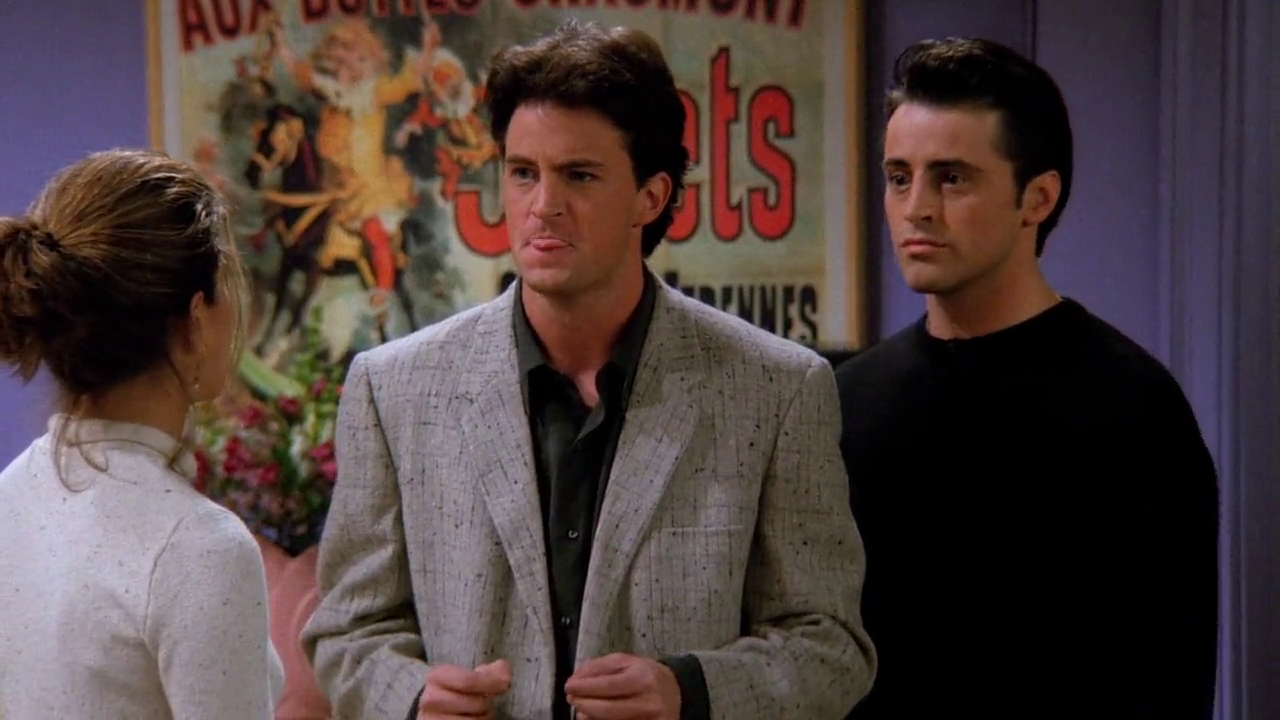
\includegraphics[trim={0 11cm 0 1cm,}, clip, width=\paperwidth]{./S01/img/19/cats-and-russian-tea-room.png}
    % \caption{Cats and Russian Tea Room\label{fig:cats-and-russian-tea-room}}
  \end{adjustwidth}
\end{figure}

\begin{tcolorbox}[enhanced,center upper,
    drop fuzzy shadow southeast, boxrule=0.3pt,
    lower separated=false, breakable,
    colframe=black!30!dialogoBorder,colback=white]
\begin{minipage}[c]{0.16\linewidth}
  \raisebox{\dimexpr-\height+\ht\strutbox\relax}{
    \centering 
\includegraphics[width=1.4cm]{./assets/img/joey.png}
  }
   & \centering \scriptsize{Joey}
\end{minipage}
\hfill
\begin{minipage}[c]{0.8\linewidth}
  \textbf{- You're a monkey, you're loose in the city. Where do you go?}\\
  - Você é um macaco, que está perdido na cidade. Pra onde você vai?
\end{minipage}

\medskip
\begin{minipage}[c]{0.16\linewidth}
  \raisebox{\dimexpr-\height+\ht\strutbox\relax}{
    \centering 
\includegraphics[width=1.4cm]{./assets/img/chandler.png}
  }
   & \centering \scriptsize{Chandler}
\end{minipage}
\hfill
\begin{minipage}[c]{0.8\linewidth}
  \textbf{- Okay, it's his first time out, so he's probably gonna want to do some of the touristy things. I'll go to Cats. You go to the Russian Tea Room.}\\
  - Tá, é a primeira vez dele fora, ele provavelmente vai pra pontos turísticos. Eu vou ao Cats. Vocês vão ao Russian Tea Room.
\end{minipage}
\end{tcolorbox}

Marcel fugiu e Joey tenta sugerir uma forma de encontrá-lo. Chandler faz
pouco e menciona que ele pode ter ido a dois locais turísticos:
\emph{Cats} e o \emph{Russian Tea Room}. \emph{Cats} (1981) é um musical
que estreou em Londres e que, logo no ano seguinte, se tornou o evento
do ano da \emph{Broadway}.\footnote{\sloppy An oral history of Cats on Broadway - Vulture (Inglês). \url{https://bit.ly/3lvM3rk}}
\emph{Russian Tea Room} (1927) é um restaurante de arquiterura no estilo
Russo fundado por membros do \emph{Balé Imperial Russo}.\footnote{\sloppy Russian Tea Room - Site oficial. \url{https://russiantearoomnyc.com/about/}}

\hypertarget{regis-philbin}{%
\section{Regis Philbin}\label{regis-philbin}}

\begin{figure}[!ht]
  \begin{adjustwidth}{-\oddsidemargin-1in}{-\rightmargin}
    \centering
    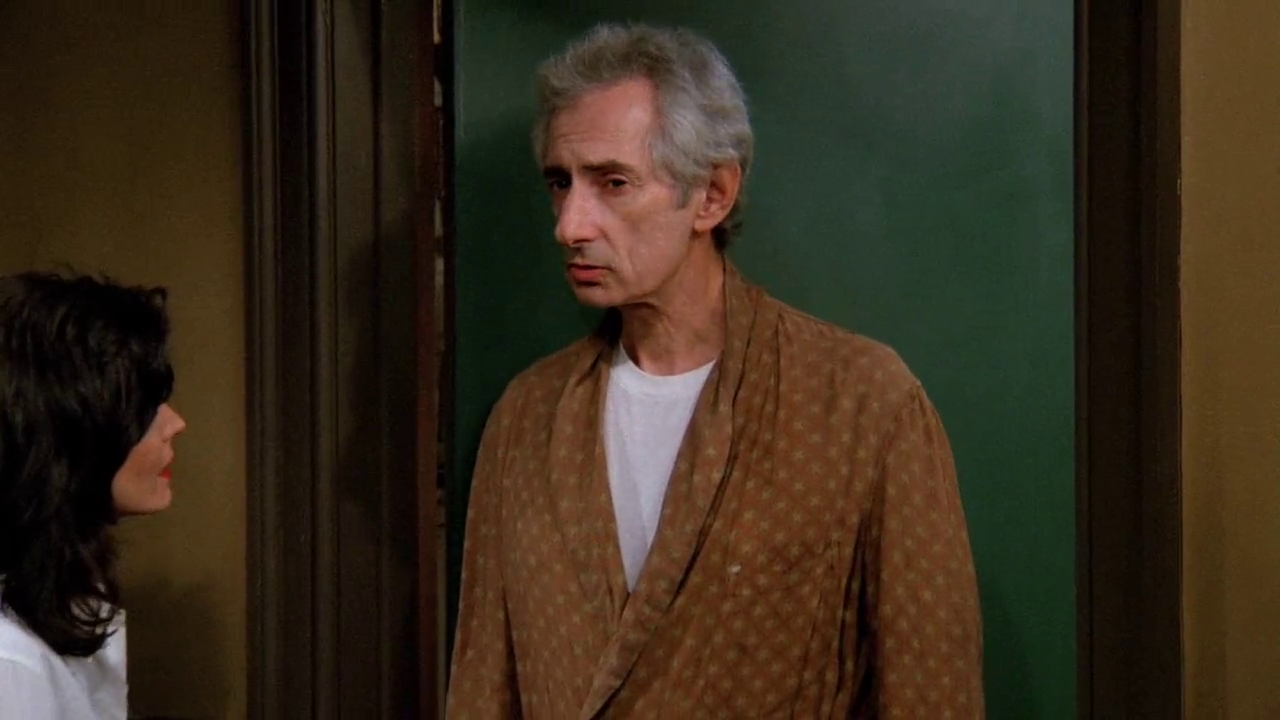
\includegraphics[trim={0 7cm 0 0cm,}, clip, width=\paperwidth]{./S01/img/19/regis-philbin.png}
    % \caption{Regis Philbin\label{fig:regis-philbin}}
  \end{adjustwidth}
\end{figure}

\begin{tcolorbox}[enhanced,center upper,
    drop fuzzy shadow southeast, boxrule=0.3pt,
    lower separated=false, breakable,
    colframe=black!30!dialogoBorder,colback=white]
\begin{minipage}[c]{0.16\linewidth}
  \raisebox{\dimexpr-\height+\ht\strutbox\relax}{
    \centering 
\includegraphics[width=1.4cm]{./assets/img/monica.png}
  }
   & \centering \scriptsize{Monica}
\end{minipage}
\hfill
\begin{minipage}[c]{0.8\linewidth}
  \textbf{- The monkey, have you seen a monkey?}\\
  - O macaco, você viu um macaco?
\end{minipage}

\medskip
\begin{minipage}[c]{0.16\linewidth}
  \raisebox{\dimexpr-\height+\ht\strutbox\relax}{
    \centering 
\includegraphics[width=1.4cm]{./assets/img/heckles.png}
  }
   & \centering \scriptsize{Heckles}
\end{minipage}
\hfill
\begin{minipage}[c]{0.8\linewidth}
  \textbf{- I saw Regis Philbin once.}\\
  - Eu vi Regis Philbin uma vez.
\end{minipage}
\end{tcolorbox}

Ao ser questionado sobre o paradeiro de Marcel, Mr.~Heckles faz
referência ao apresentador \emph{Regis Philbin} (1931-2020), conhecido
principalmente por apresentar o programa \emph{Who Wants to Be a
Millionaire} (1998), \emph{game show} em que o participante deve
responder uma série de perguntas de múltipla escolha. Uma versão do
programa foi desenvolvida por \emph{Silvio Santos}, chamada \emph{Show
do Milhão} (1999-2003).\footnote{\sloppy Regis Philbin - Biography (Inglês). \url{https://www.biography.com/personality/regis-philbin}}

\hypertarget{von-trapp-kids}{%
\section{Von Trapp Kids}\label{von-trapp-kids}}

\begin{figure}[!ht]
  \begin{adjustwidth}{-\oddsidemargin-1in}{-\rightmargin}
    \centering
    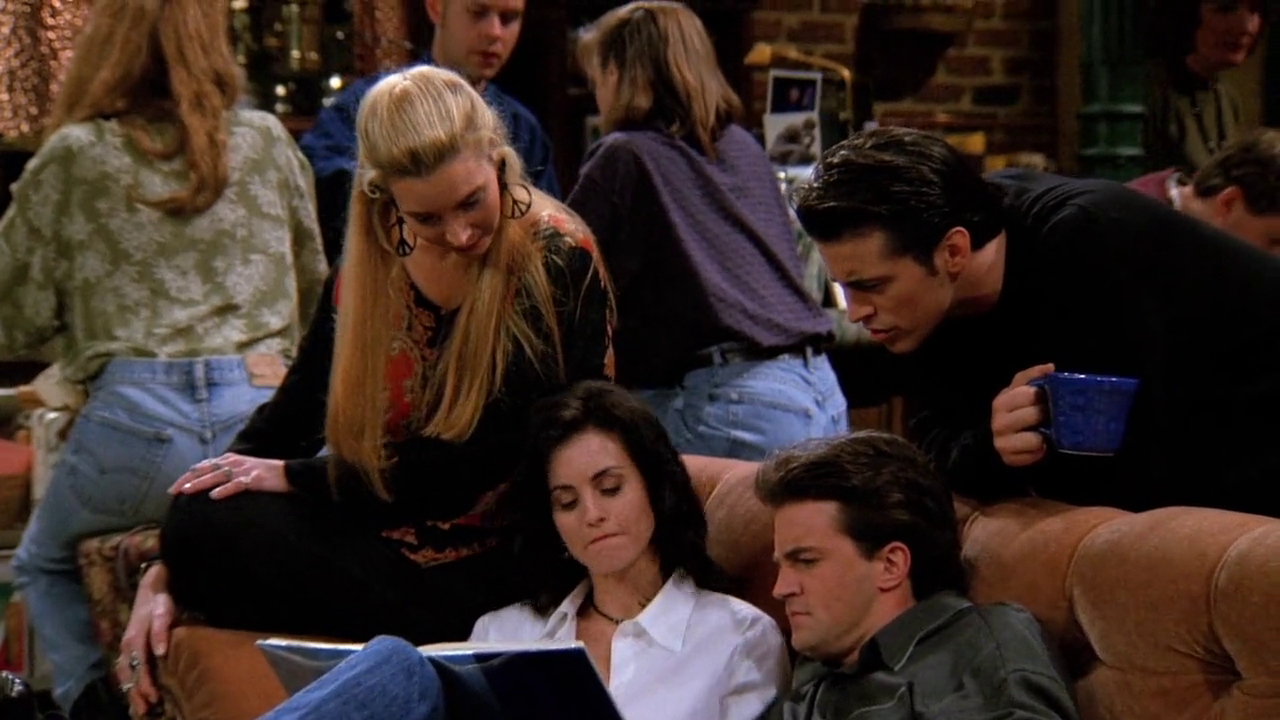
\includegraphics[trim={0 0cm 0 3cm,}, clip, width=\paperwidth]{./S01/img/19/von-trapp-kids.png}
    % \caption{Von Trapp Kids\label{fig:von-trapp-kids}}
  \end{adjustwidth}
\end{figure}

\begin{tcolorbox}[enhanced,center upper,
    drop fuzzy shadow southeast, boxrule=0.3pt,
    lower separated=false, breakable,
    colframe=black!30!dialogoBorder,colback=white]
\begin{minipage}[c]{0.16\linewidth}
  \raisebox{\dimexpr-\height+\ht\strutbox\relax}{
    \centering 
\includegraphics[width=1.4cm]{./assets/img/monica.png}
  }
   & \centering \scriptsize{Monica}
\end{minipage}
\hfill
\begin{minipage}[c]{0.8\linewidth}
  \textbf{- This is me in The Sound of Music. You see the von Trapp kids?}\\
  - Esta sou eu no The Sound of Music. Conseguem ver as crianças von Trapp?
\end{minipage}

\medskip
\begin{minipage}[c]{0.16\linewidth}
  \raisebox{\dimexpr-\height+\ht\strutbox\relax}{
    \centering 
\includegraphics[width=1.4cm]{./assets/img/phoebe.png}
  }
   & \centering \scriptsize{Phoebe}
\end{minipage}
\hfill
\begin{minipage}[c]{0.8\linewidth}
  \textbf{- No.}\\
  - Não.
\end{minipage}

\medskip
\begin{minipage}[c]{0.16\linewidth}
  \raisebox{\dimexpr-\height+\ht\strutbox\relax}{
    \centering 
\includegraphics[width=1.4cm]{./assets/img/monica.png}
  }
   & \centering \scriptsize{Monica}
\end{minipage}
\hfill
\begin{minipage}[c]{0.8\linewidth}
  \textbf{- That's because I'm in front of them.}\\
  - É porque estou na frente delas.
\end{minipage}
\end{tcolorbox}

Mostrando fotos de seu anuário, Monica descreve o que parece ser uma
encenação teatral do musical \emph{The Sound of Music} (1959), e faz
referência a \emph{Von Trapp kids}. Na história --- baseada no livro
\emph{The Story of the Trapp Family Singers} (1949) --- Maria se
apaixona por Georg, que era viúvo e tinha sete crianças.\footnote{\sloppy The von Trapps - Biography (Inglês). \url{https://www.biography.com/news/real-von-trapp-family-sound-of-music}}

O musical \emph{The Sound of Music} já foi citado em
\textbf{\textcolor{primarycolor}{S01E01 - Aquele onde Tudo começou}}.
